\documentclass[a4paper,12pt]{article}
\usepackage{fullpage}
\usepackage{graphicx}
\usepackage{caption}
\usepackage{float}
\usepackage{hyperref}

\hypersetup{
    colorlinks,
    citecolor=blue,
    filecolor=black,
    linkcolor=blue,
    urlcolor=blue
}
\begin{document}
%\selectlanguage{english}
\pagenumbering{Roman}



\title{\begin{Huge}
\textbf{Software Requirements Specification: Simulation Platform for Smart Fridge and Sudoku Solver}
\end{Huge}}
\author{\begin{Large}
Sreenivas, Jonas and Mariusz
\end{Large}}
\date{\today}
\maketitle
\thispagestyle{empty}
\begin{center}
\begin{large}
\textbf{Version:} 1.0
\\  \textbf{Based on:} IEEE SRS Template
\end{large}
\end{center}
\newpage
\tableofcontents \newpage
\pagenumbering{arabic}
\section{Introduction}
\subsection{Purpose}
This document is a software requirement specification for the simulation platform which is built to aid the SmartFridge and Sudoku solver projects by providing simulated data.
\subsection{Document Conventions}
\begin{itemize}
\item Links are marked in blue color and are accessible through the web browser.
\item Reference titles are in italics for easier viewing
\end{itemize}
\subsection{Intended Audience and Reading Suggestions}
The document is intended for the Systems and Software Engineering lecture (WS 2017-18) at Goethe University. This document is also intended for developers and document writers of our related projects: SmartFridge and sudoku solver. The document should be read completely in order and it is preferred to read through the documents of the related projects to get better understanding.
\subsection{Product Scope}
A software platform for generating images which could be used as a dataset for other projects. For understanding the scope of the other projects, please refer to smart fridge software requirements specification document.
\subsection{References}
\begin{itemize}
\item IEEE, \textit{Software Requirements Specification}. Available at \url{https://view.officeapps.live.com/op/view.aspx?src=https://web.cs.dal.ca/~hawkey/3130/srs_template-ieee.doc}
\item Stuart R. Faulk, \textit{Software Requirements: A Tutorial}, 1995. Available at \url{http://citeseerx.ist.psu.edu/viewdoc/download?doi=10.1.1.198.7770&rep=rep1&type=pdf}
\end{itemize}
\newpage
\section{Overall Description}
\subsection{Product Perspective}
It is a self contained project that can be used to simulate a large amount of data, which can potentially be used by developers, testers and users who wish to simulate images. These images include vegetables (in specific banana, tomatoes, apples and grapes) both in rotten and non-rotten form and sudoku puzzles with varying transformation and noise to evaluate other projects that require simulated data.

\subsection{Product Functions}
\begin{itemize}
\item User gives context for his application which we use in our simulation platform
\item The simulation platform generates a huge dataset of images with labels based on the context.
\end{itemize}

\begin{figure}[H]
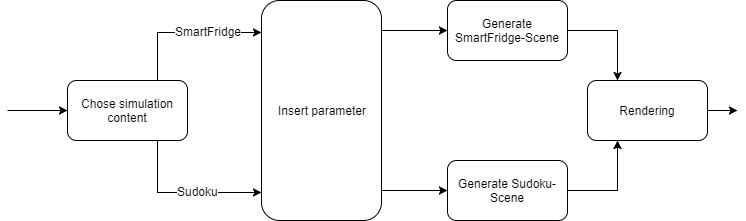
\includegraphics[scale=0.6]{sys_sw.png}
\end{figure}
\subsection{User Classes and Characteristics}
\begin{itemize}
\item Developers and testers: Use simulated data for testing their algorithms
\item Others: Create fancy simulated images.
\end{itemize}
\subsection{Operating Environment}
The generated images should be readable and useful for other projects which use this to test their algorithms. The software should run on Linux and/or Microsoft Windows. The results should be readable on all major Operating Systems.
\subsection{Design and Implementation Constraints}
\begin{itemize}
\item Complexity of the model in context to simulate is a constraint for the developers.
\item The software should run on a laptop with average capabilities.
\item Users/Customers should know how to run simple exe files or commands from the terminal and have basic knowledge on their system's capabilties.

\end{itemize}
\subsection{User Documentation}
The following documents will be given to the user:
\begin{itemize}
\item User Manual.
\item Troubleshooting, FAQs.
\item Tutorials and samples.
\end{itemize}
\subsection{Assumption and Dependencies}
This particular software depends on open sourced simulation platforms such as Blender, Unreal Engine.
\newpage
\section{External Interface Requirements}
\subsection{User Interfaces}
The software provides a simple user interface as shown below:
\begin{figure}[H]
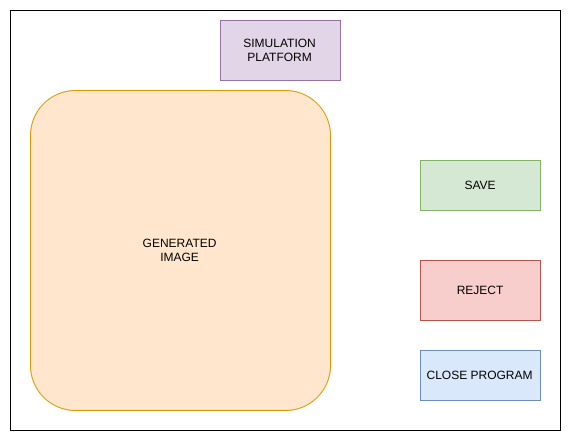
\includegraphics[scale=0.75]{gui.png}
\end{figure}
\subsection{Hardware Interfaces}
The systems works stand alone and the generated results are stored on the same hardware device.
\subsection{Software Interfaces}
The dataset generated from the hardware is passed on as an image data. 

\newpage
\section{System Features}
\subsection{Generate Images}
This feature pertains to generating a dataset of rendered images. It has high priority.


\subsubsection{Stimulus/Response Sequences}
\begin{itemize}
\item User runs the software.
\item User chooses to select or reject the generated image.
\end{itemize}
\subsubsection{Functional Requirements}
\begin{itemize}
\item \textbf{REQ-1:} Simulate images based on the requirements from the projects: SmartFridge and Sudoku solver.
\item \textbf{REQ-2:} Display images for user interaction.
\item \textbf{REQ-3:} Provide labels/annotations for selected images by the user.
\item \textbf{REQ-4:} Saving the selected images for future use.
\end{itemize}
\section{Other Nonfunctional Requirements}
\subsection{Performance Requirements}
\begin{itemize}
\item \textbf{REQ N-1.1:} Must run on a single core CPU with/without a GPU.
\end{itemize}

\subsection{Software Quality Attributes}
\begin{itemize}
\item \textbf{REQ N-2.1:} The software should be portable across systems and platforms.
\item \textbf{REQ N-2.2:} The software must be reliable enough such that there is not a huge disparity between the results generated from simulations and real images.
\end{itemize}

\section{Other Requirements}
In terms of license, we use GNU General Public License v2.0. The software can be used commercially, modified, distributed and can be used privately. We do not provide any liability or warranty for the software.
\end{document}
